For critical systems, it has been argued that formal methods
%, involving formalized requirements and proofs of implementation correctness,
should be applied to gain higher assurance than is possible with testing~\cite{Miller10:CACM,Rushby09:SEFM,Hardin09:Security}.  For these approaches, testing may still be performed, but the verification effort is primarily focused on performing proofs.  Unfortunately, proof-based approaches tend not to answer the question as to whether implementations have {\em additional functionality} that is not covered by requirements.  Testing, despite its faults, can measure {\em structural coverage} to find untested functionality and can find some errors by {\em serendipity}, in which problems not directly related to the requirement under test are exposed.  Therefore, in formal verification approaches, it is even more important that requirements be complete.

In general, specification completeness can be defined with
regard to the notion of coverage. In fact, the way that coverage
is formalized plays a key part in the strength/effectiveness of
a method for the assessment of completeness. The goal of a coverage metric is usually to assign a numeric score that describes how well properties cover the design.
Relatively recently, techniques have been devised for analyzing completeness of requirements against formal implementation models, specified as transition systems or Kripke structures \cite{chockler2001practical,das2005formal, claessen2007coverage, grosse2007estimating}.  These models are agnostic to the abstraction level of the implementation: implementations can be lower-level requirements, software architectures, or concrete implementations of system behavior.  The mechanism used is based on {\em mutation} and {\em proof}: is it possible to prove that the requirements still hold of the system after mutating the model in some way?  If so, then the requirements are incomplete with respect to that model element. Mutations are ``atomic'' changes to the design, where the set of possible mutations depends on the notation that is used.  A mutant is ``killed'' if one of the properties that is satisfied by the original design is violated by the mutated design~\cite{chockler_coverage_2003,chockler2001practical,chockler2010coverage,Kupferman:2006:SCF,kupferman_theory_2008}.  There are many different kinds of mutations that have been proposed, primarily focused on checking sequential bit-level hardware designs.
For these designs, {\em State-based} mutations flip the value of one of the bits in the state.  There are several variations depending on whether the flip is performed on a single state within a Kripke structure~\cite{hoskote1999coverage}, or in the description of the signal in the transition relation of the circuit~\cite{chockler2001practical}.  {\em Logic-based} mutations fix the value of a bit to constant zero or one, and can be used to determine whether properties can find stuck-at faults.  {\em Syntactic} mutations~\cite{chockler_coverage_2003} remove states in a control flow graph representation of hardware.
Similarly, for software, it is possible to apply any of the ``standard'' source code mutation operators used for software testing~\cite{Andrews06:mutation} towards requirements coverage analysis.
Some examples of software mutations are \cite{Budd:1980}:
\begin{enumerate}
    \item Replace an integer constant $C$ by one of $\{0, 1, -1, C + 1, C - 1\}$,
    \item Replace an arithmetic, relational, logical, bitwise logical, increment/decrement, or arithmetic-assignment operator by another operator from the same class,
    \item Negate the decision in an \texttt{if} or \texttt{while} statement,
    \item Delete a statement.
\end{enumerate}

We assume each element $T_i \in T$ has a set of possible mutations associated with it.  Depending on the modeling formalism used, this may be the value of a gate or signal or an expression within a statement in a program.  We will further assume the existence of a mutation function $f_{m}$ that, given a model element, will return a finite set of mutations for that element.  We can then define the set of mutant models $M$ as follows:
\[
    M = \{ (T \setminus \{T_i\}) \cup \{m\} \ |\ T_i \in T, m \in f_{m}(T_i) \}
\]
\noindent and then define the mutation score for property $P$ in the standard way:
\begin{definition} {\emph{Generalized mutation coverage.} } \\
\[
   \mutcov = \frac{ | \{m~|~ m \in M~\land~(I, m) \nvdash P\} |}{|M|}
\]
\end{definition}

\noindent Note that without loss of generality, we consider a single property $P$, which can be viewed as the conjunction of all the properties of the model.

The state of the art of mutation-based coverage can be found in Chockler \textit{et al.} \cite{chockler2010coverage}, where a design is considered as a net-list with nodes of types {\small \texttt{\{AND, INVERTER, REGISTER, INPUT\}}}.
Each mutant design changes the type of a single node to {\small \texttt{INPUT}}. When property $\phi$ satisfied by the original net-list fails on the mutant design, it is said that a mutant is discovered for $\phi$. Then, the coverage metric for $\phi$ is defined as the fraction of the discovered mutants, based on which the coverage of a set of properties is measured as the fraction of mutants discovered by at least one property.
To decrease the cost of computation, coverage analysis is performed at several stages; first, all the nodes that do not appear in the resolution proof of a given property are marked as \emph{not-covered}, and the rest of the nodes are marked as \emph{unknown}. Then, for the unknown nodes, the basic mutation check is performed: if a corresponding mutant design violates the property, it will be considered as \emph{covered}.

Unfortunately, previous completeness metrics can {\em underapproximate} which portions of a program are necessary to fulfill the requirements.  That is, if we construct a model consisting of only the required model elements as determined by the analysis, it is often no longer possible to prove the requirement.  Thus the feedback provided to the developer may be somewhat misleading.  In addition, the mutation-based analyses tend to be very computationally expensive.  For example, for model checkers, state of the art techniques have runtimes of (in the best case) several times more than is required for proof~\cite{chockler2010coverage}. We propose a new approach for measuring property completeness based on proof rather than mutation.


%\footnote{Section~\ref{sec:impl} describes how these proofs are discovered in practice.}
%\subsection{Coverage and Minimal Proofs}
%Alternatively, we can consider using the proofs themselves as a mechanism for determining adequacy of requirements.

\begin{definition} {\emph{IVC coverage (\ivccov):}} \\
\label{def:coverage-justi}
Given $S \in \aivc(P)$, $T_i$ is covered by $P$ via $S$ \emph{iff} $T_i \in S$.
\end{definition}

We call Definition \ref{def:coverage-justi} a \emph{proof-preserving} metric because, with a set of the model elements marked as covered by \ivccov ,
$P$ is provable.  Other notions, as will be discussed,
may yield subsets of the model that are insufficient to
reconstruct the proof of the property.
%\footnote{\noindent ~Throughout the paper, when a coverage metric is justifiable, like \ivccov, we say that it preserves provability of the property.}
%Thus, the coverage score for \ivccov\ is often higher than the score for \nondetcov.
The coverage score for \ivccov\ can be calculated with: $$\frac{|S|}{|T|}$$
%Note that because minimal proofs are not unique, there are several possible coverage scores.
Because $P$ may have multiple \mivc s,
  \ivccov\ metric can lead to various scores that belong to the following set:
\[
<<<<<<< HEAD
\Big{~\frac{ |S|}{|T|}~|~S \in AIVC(P)~\Big}
=======
\{~\frac{ |S|}{|T|}~|~S \in \aivc(P)~\}
>>>>>>> 55ab1992dbd6e96cf965abe1ee03f1c21467bd70
\]

\noindent Note that if an \mivc ~contains all model elements (i.e., the model is {\em completely covered}), then there is only one possible \mivc , so in this case there is no diversity of scores. On the other hand, a set of states and signals can be considered covered or not covered depending on a particular \mivc\ we consider for coverage evaluation. To address this issue, we introduce additional coverage metrics using the notions of \may\ and \must.

%the model is {\em completely covered}, on the other hand, then there is only one possible minimal set: the set of all elements.

<<<<<<< HEAD
Using the notions of \textit{MAY} and \textit{MUST}, we can introduce additional coverage metrics.
=======

>>>>>>> 55ab1992dbd6e96cf965abe1ee03f1c21467bd70
%Since the primary goal of
% this paper has been to provide a complementary coverage notion in
%  formal verification, it is worth exploring other possible notions based on the idea of provability and $\aivc$, which is beneficial, as with testing, because if a coverage notion is an over-approximation, when the coverage
% is high, it does not necessarily mean the quality of
% the specification (or test suite) is high, or when it is an under-approximation, a low coverage score does not always mean the specification is of poor quality.

\begin{definition} {\emph{(\maycov):}}
  \label{def:comp-1}
 $T_i \in T$ is covered by $P$ \emph{iff} $T_i \in \maycov (P)$, where
   $\maycov (P) = \{T_i ~|~ \exists S \in \aivc(P)~.~T_i \in S \}$.
\end{definition}

\begin{definition} {\emph{(\mustcov):}}
  \label{def:mustcov}
 $T_i \in T$ is covered by $P$ \emph{iff} $T_i \in \mustcov (P)$, where
   $\mustcov (P) = \{T_i ~|~ \forall S \in \aivc(P)~.~T_i \in S \}$.
\end{definition}

The $\maycov$ notion aims to deal with the fact that a property $P$ may have
several distinct {\mivc}s. In such cases, \ivccov\ only looks at an arbitrary \mivc\
that may contain a subset of $\may(P)$, which means, depending on
which \mivc\ it considers, every time it may report a different part of $\may(P)$
as uncovered. However, \maycov\ resolves this issue reporting the entire set of $\may(P)$ as covered, which also leads to higher coverage scores.  \mustcov\ takes the opposite view, considering a model element as covered only if it affects all the proofs of $P$.
Algorithm \ref{alg:must} is also an efficient way of computing the \emph{must} set of a given property using \ucalg. A different algorithm for computing $\must (P)$ is to first compute $\aivc (P)$ and then take the intersection of all sets in $\aivc (P)$.


\begin{algorithm}
  \SetKwInOut{Input}{input}
  \SetKwInOut{Output}{output}
  \Input{$(I, T) \vdash P$}
  \Output{Must set for $(I, T) \vdash P$}
  \BlankLine
  $S \leftarrow \ucalg((I, T) \vdash P)$ \\
  $M \leftarrow \varnothing$ \\
  \For{$x \in S$} {
    \If{$(I, T\setminus\{x\}) \nvdash P$}{
      $M = M \cup \{x\}$
    }
  }
  \Return{M}
\caption{\mustalg: an algorithm to compute $\must(P)$ for a given $P$}
\label{alg:must}
\end{algorithm}

It is still possible to build more relaxed coverage metrics in which coverage
is captured by looking at individual properties, rather than their conjunction.
%for example, in the definition of \ivccov , it is wise to look at $P$ as
%the conjunction of all properties. However,
We can, for example, describe a metric in which any element used by an \mivc ~for any property is considered covered.
%with this view,
%elements around IVCs that do not have common \emph{must}
%elements with others will be treated as uncovered while they are at least covered by one
% IVC of an individual property in the specification.
%
The next definition, \allcov, formalizes this notion.
\begin{definition} {\emph{(\allcov):}}
  \label{def:comp-2}
     Given a set of properties $\Delta$ over $T$, $T_i \in T$ is covered
   \emph{iff} $T_i \in \allcov (T)$, where
   $\allcov (T) = \{T_i ~|~ \exists P \in \Delta ,~ S \in \aivc(P).~T_i \in S \}$.
\end{definition}

Based on the categorization of elements, we will state some relationships about \mivc s in order to compare different proof-based metrics proposed earlier.

\begin{lemma}
  \label{lem:must-not-enough}
  If $\may(P) \neq \varnothing$, then $P$ is not provable by $\must(P)$.
\end{lemma}
\begin{proof}
  $\may(P) \neq \varnothing \Rightarrow  \exists T_i \in \may(P).$
$T_i \in \bigcup \aivc(P) \wedge T_i \notin \must(P)$,
which implies $\exists S \in \aivc(P).~ T_i \in S$.
Considering the fact that $S$ is minimal and
$\must(P) \subset S$ (since $T_i \in S \wedge T_i \notin \must(P)$),
 $\nexists S' \subset S.~ (I,S') \vdash P$,  which means $(I, \must(P)) \nvdash P$.
\end{proof}
\vspace{2mm}

%\begin{lemma}
%    \label{lem:must-mustcov}
%    $T_i \in \must(P) \Leftrightarrow T_i \in \mustcov(P)$
%\end{lemma}
%\begin{proof}
%Immediate from the definition of $\must$ and \mustcov.
%\end{proof}

Now we focus on the relationship between non-deterministic mutation-based coverage and proof-based metrics. In Chockler et. al.
~\cite{chockler2010coverage},
each mutant design changes the type of a single node to an input node .
Given a suitable encoding of the netlist, assigning a ``fresh'' input is an isomorphic operation to simply removing a $T_i$ from $T$. The mapping is as follows: the net-list becomes a conjunction
of equations, where each vertex becomes a variable $v_i \in U$, and where each non-input vertex becomes an assignment equation $T_i \in T$.
For example, given an AND-vertex $v_i$ with three input edges from other vertexes $\{v_a, v_b, v_c\}$, we would define an equation $T_i \in T$ of the form $(v_i = (v_a \wedge v_b \wedge v_c))$.
%
%As the variable is no longer constrained by a defining equation, it is effectively an %input.

Given this encoding, we can reframe the non-deterministic coverage proposed in \cite{chockler2010coverage} as follows:

\begin{definition} {\emph{Nondeterministic coverage (alternate specification) (\nondetcovalt) ~\cite{chockler2010coverage}.} }
\label{def:non-det-2}
$T_i \in T$ is covered by property $P$ \emph{iff} $T_i \in \nondetcovalt (P)$, where
$\nondetcovalt (P) = \{T_i~|~ (I, T) \vdash P \wedge (I, T \setminus \{T_i\}) \nvdash P\}$.
\end{definition}
\noindent Given this definition, it becomes straightforward to define some additional properties.

\begin{lemma}
  \label{lem:must-coverage}
$T_i \in \nondetcovalt (P) \Leftrightarrow T_i \in \mustcov(P)$.
\end{lemma}
\begin{proof}
$T_i \in \nondetcovalt (P)$ means that $(I, T \setminus \{ T_i \}) \nvdash P$ then
%$T_i$ is necessary to prove $P$,  which means
$\forall S \subset T .~ T_i \notin S \Rightarrow (I, S) \nvdash P$.
Therefore, since $(I, T) \vdash P$, $T_i \in \bigcap \aivc(P)$, which means  $T_i \in \must(P)$.
On the other hand, let $T_i \in \must(P)$; then $\forall S \in \aivc(P).~ T_i \in S$.
By definition, any proof of $P$ is a superset of some minimal IVC in $\aivc(P)$.
Thus, any subset $S$ of $T$ leading to proof contains $T_i$.
Therefore, $T \setminus \{ T_i \}$ does not lead to a proof.

\end{proof}
\vspace{2mm}

In light of Lemma \ref{lem:must-coverage}, the \nondetcovalt\ coverage score of specification $P$ can be also calculated by
$$\frac{|\must(P)|}{|T|}$$
%Therefore, for set of properties $\Delta$, the coverage score is computed by $$\frac{|\must(\Pi)|}{|T|},\quad  \Pi= \bigwedge_{i} {P_i \in \Delta}$$


%\mike{after all metrics presented, contrast them on the example.  Introduce the properties HERE and then discuss the coverage sets}
%
%\mike{Then, you can talk about justification, etc.}
\begin{corollary}
\label{cor:must-not-provable}
\nondetcovalt\ is not proof-preserving.
\end{corollary}
\begin{proof}
Immediate from Lemma \ref{lem:must-not-enough} and Lemma \ref{lem:must-coverage}
\end{proof}
\vspace{2mm}
\begin{corollary}
\label{cor:ivc-provable}
\ivccov\ is proof-preserving.
\end{corollary}
\begin{proof}
Immediate from Definition~\ref{def:minimal-ivc} and Definition \ref{def:coverage-justi}
\end{proof}
\vspace{2mm}

%It should be pointed out that \ivccov\ is accurate meaning that it does not result in false positives. In other words, since IVCs are \emph{minimal}, \ivccov\ does not mark
%any \emph{actual} uncovered element as covered.

To conclude this section, we should mention that one can define many more proof-based coverage metrics based on the $\mivc$s and $\aivc$s.  Metrics that make use of the $\aivc$ relation are computationally more expensive than \ivccov.

Figure~\ref{fig:runtimeall} allows a visualization of the runtime of different coverage analyses
in comparison with the proof time, which indicates the overhead induced by each algorithm.
As can be seen, it is computationally cheap to find an
approximately minimal IVC using the algorithm \ucalg; however, finding a {\em guaranteed}
minimal IVC using the \ucbfalg\ algorithm is computationally expensive. The overhead of the \ucalg\ algorithm is on average 31\% over the baseline proof, as opposed to 2276\% for the \ucbfalg\ algorithm.
Therefore, in order to compute \ivccov, it is much more efficient to use \ucalg\ rather than the \ucbfalg\ algorithm.
In terms of comparing cost of coverage computation from \ivccov\ and \mustcov ,
the \mustcov\ computation imposes an average 4183\% runtime overhead on the verification time.


\begin{figure}
  \centering
  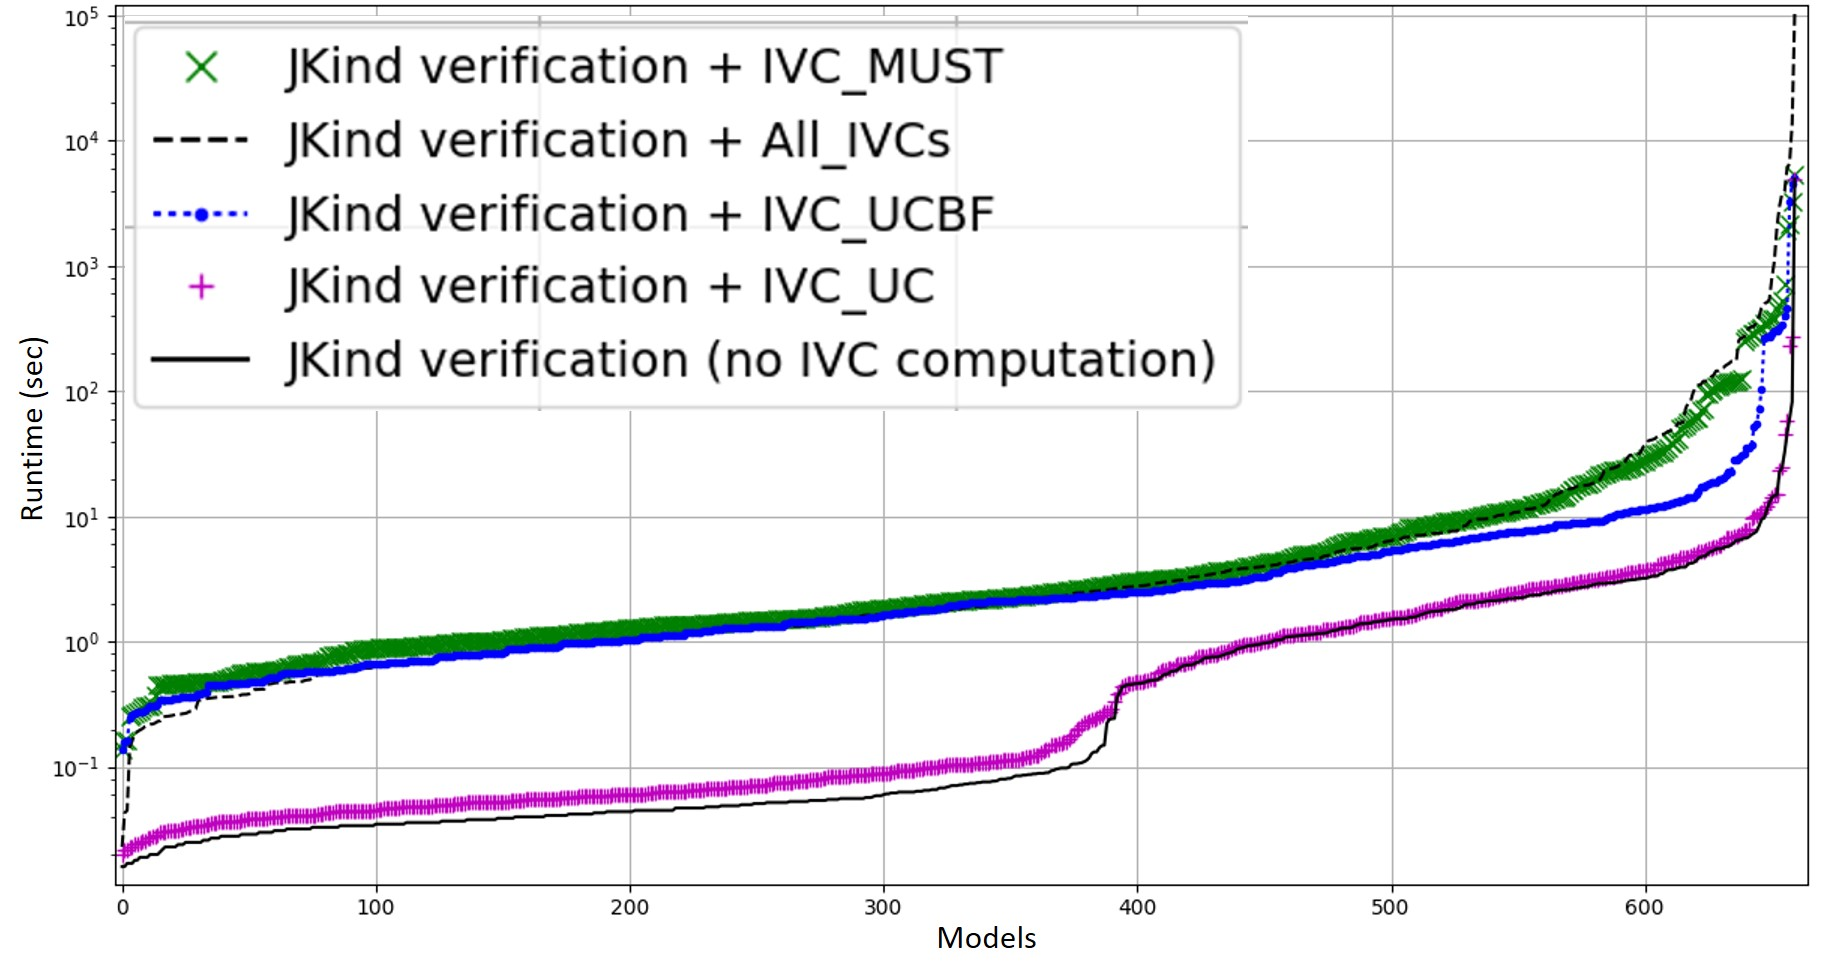
\includegraphics[width=\columnwidth]{figs/timing_cv.jpg}
  %\vspace{-0.2in}
  \caption{Runtime of different analyses}\label{fig:runtimeall}
\end{figure}


\begin{figure}
  \centering
  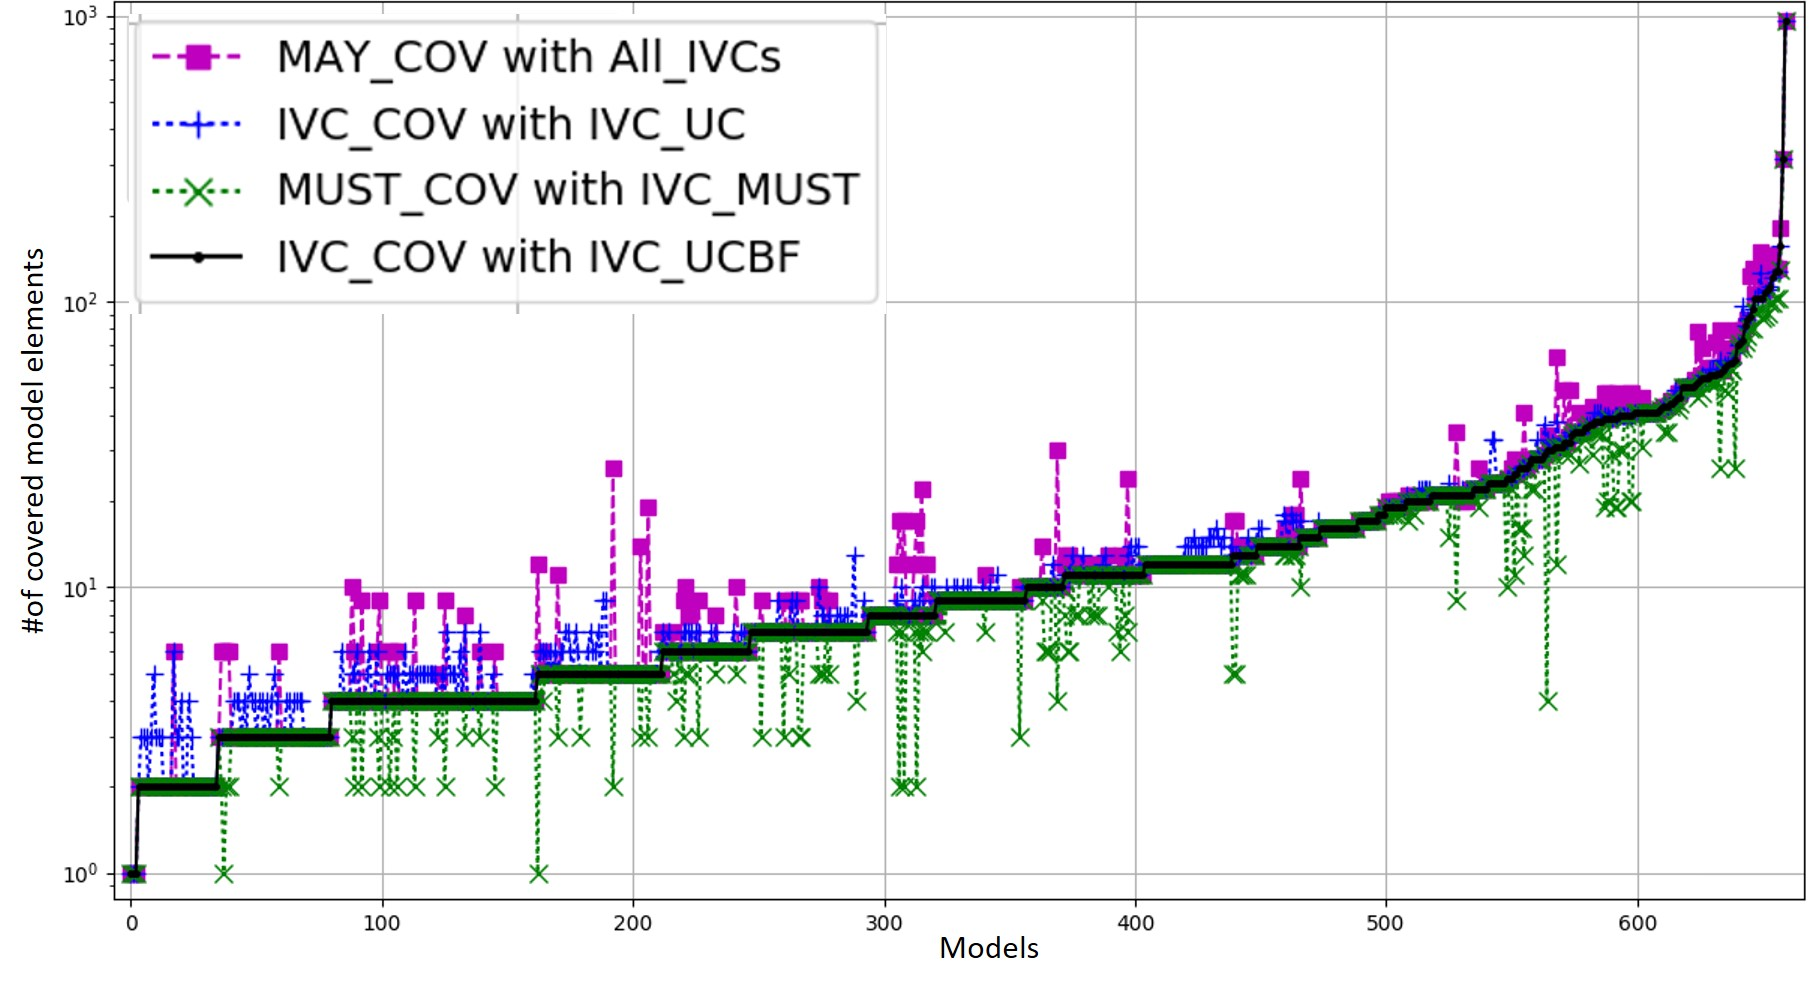
\includegraphics[width=\columnwidth]{figs/cv_size.jpg}
  %\vspace{-0.2in}
  \caption{Size of the set of covered elements by different algorithms}\label{fig:cvsize}
\end{figure}

When a coverage metric brings about lower coverage scores on average,
it is said that the metric is harder to satisfy.
To study this aspect of the proposed metrics,
we first calculated the size of the output sets generated by each algorithm: on average, the ratio of the size of the sets generated by \ucalg\ to the size of the ones obtained from \ucbfalg\ is 1.08,
while this ratio for \mustalg\ to \ucbfalg\ is 0.93, which shows \mustalg\ is harder to satisfy, and also is not proof-preserving.

Figure \ref{fig:cvsize} is a visualization of the size of the set of covered elements by different algorithms. Models over the x-axis are sorted based on the size of the minimal IVCs obtained from the \ucbfalg\
algorithm.
The graph shows the degree of under-approximation of a minimal proof set by \mustalg\ as well as the degree of over-approximation by \ucalg.
Moreover, the size of sets computed by \ucalg\ is very close to the size
of the ones obtained from \ucbfalg, especially for larger models.  The average increase in size of IVCs returned by \ucalg\ is approximately 8\% of the \ucbfalg\ algorithm.  Since the overhead of producing \ucalg\ is only approximately 31\% more expensive than the baseline analysis, this test may be efficient enough to run as a standard part of the model checking process.  %If guaranteed minimality is required, the \ucbfalg\ can be used, but


%For many analysis problems, this may be accurate enough to

%, which makes \ucalg a reasonable choice for computing \ivccov ~(rather than using \ucbfalg ).
%Therefore, minimality does not dramatically
%affect the coverage scores when \ivccov\ is computed by the \ucalg\ rather than \ucbfalg.
%However, \ucalg might report some elements as covered, while they are not because of the minimality issue.
%And, \mustalg reports some elements uncovered, while they are because it is not able to find \emph{may} elements.

Table~\ref{tab:cov-score} describes the aggregate of the coverage scores returned by the analyses.  Across all benchmarks, the min and max coverage scores are the same, and as expected, the average number of elements required is smallest for the \mustalg\ algorithm and largest the for \ucalg\ algorithm.

\begin{table}
  \caption{Coverage score of different algorithms}
  \centering
  \begin{tabular}{ |c||c|c|c|c| }
    \hline
     score & min & max & mean & stddev \\[0.5ex]
    \hline\hline
    \small{\ivccov}\ with \ucalg &   0.002  & 1.0  & 0.475 & 0.302 \\[0.5ex]
    \small{\ivccov}\ with \ucbfalg&  0.002 & 1.0 &  0.445 & 0.291 \\[0.5ex]
    \mustcov & 0.002 & 1.0 &  0.417 & 0.291 \\[0.5ex]
    \maycov& 0.002 & 1.0 &  0.476 & 0.301 \\[0.5ex]
    \hline
  \end{tabular}
  \label{tab:cov-score}
\end{table}

The proposed coverage metrics can be ranked in terms of their scores as follows:
$$\nondetcovalt\ \leq \ivccov\ \leq \maycov\ \leq \allcov$$
\ivccov\ and \nondetcovalt\ are equivalent when all elements within the model are covered: if all model elements are \must elements, then there can only be one \mivc , and this \mivc ~uses all of the model elements. The equivalence of \mustcov\ and \nondetcovalt\ allows us to compare our algorithms against state-of-the-art mutation based coverage.

To investigate the relationship between provability and different coverage notions,
we were interested in the number of models in the benchmark for which
\mustalg\ resulted in the sets not equal to an MIVC (i.e. models for which
\mustalg\ did not preserve provability).
Obviously properties are provable by 100\% of the IVCs computed by \ucalg\ (and \ucbfalg).
As for the \mustalg\ algorithm, the properties of 290 models in the benchmarks were not provable by the output of \mustalg. In practice, for larger models, \mustcov\ is more likely not to maintain provability,
 and since more than half of the models are small, 43\% may still not reveal the actual degree
 to which \mustcov\ underapproximates the covered parts of a model.
  The notion of proof preservation is appealing because it allows a concrete demonstration to the user of the irrelevance of portions of the implementation.  The IVC coverage notion also allows, in cases where there are multiple minimal satisfying sets, insight on multiple ways by which the model meets a requirement.


